\section{Inicializácia algoritmov}

Na inicializáciu Metropolis--Hastings metód (Hit--and--Run generátora a aj Gibbsovho generátora) je potrebný počiatočný bod vnútri polyédra a veľkosť burn--in periódy (iterácii algoritmu bez vracania vygenerovaných bodov ako výsledkov). Ako počiatočný bod sme zvolili bod $c$ určený pri generovaní polyédra, ktorý je vygenerovaný na prieniku polyédra a jednotkovej hyperkocky rovnomerne náhodne. Vzhľadom k tomu, že generujeme veľké množstvo bodov v polyédri, je burn--in perióda nepotrebná. Symbolicky bola zvolená hodnota $100$.

Na inicializáciu zamietacej metódy pomocou MVEE elipsoidu je potrebné vypočítať MVEE elipsoid. Pri inicializácii REX algoritmu je potrebné zvoliť počiatočný nosič tak, aby bola informačná matica $M$ regulárna. V rámci práce bol nosič počiatočného návrhu zvolený ako $n+1$ náhodných vrcholov. Vzhľadom na náhodnosť polyédra, dané vrcholy budú s pravdepodobnosťou $1$ určovať regulárnu maticu $M$.

\section{Testovací algoritmus}

\textbf{TODO ráno doplniť}

\section{Porovnanie rýchlostí generovania}

V rámci testovania boli metódy porovnávané na rozmeroch $d=1, \dots, 9$, v každom rozmere bolo vygenerovaných $100$ náhodných polyédrov. Na každom z daných polyédrov boli spustené všetky metódy, každá z nich vygenerovala $10^5$ bodov vnútri polyédru. Ako výstup testovania boli pre každú metódu zobrazené priemerné rýchlosti generovaní bodov v jednotlivých rozmeroch.\\

\begin{figure} [H]
  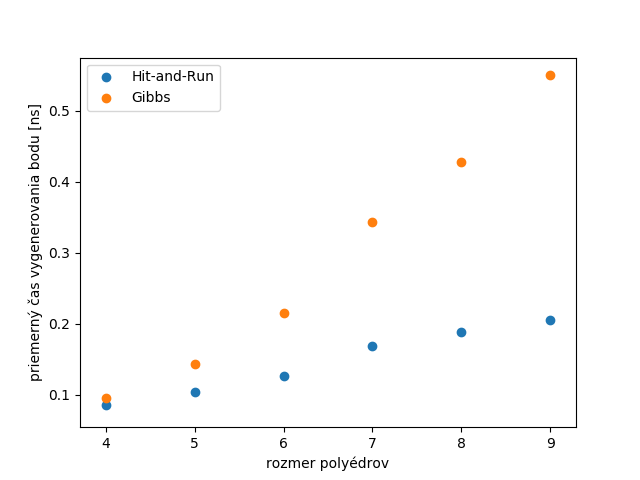
\includegraphics[width=\linewidth]{images/mh.png}
  \caption{Priemerný čas trvania generovania bodov Metropolis--Hastings metód}
  \label{fig:mh}
\end{figure}

Porovnanie Metropolis--Hastings metód dopadlo podľa očakávaní. Čas potrebný na vygenerovanie bodu pomocou Gibbsovho generátor rástol asymptoticky kvadraticky a čas potrebný na vygenerovanie bodu pomocou Hit--and--Run generátora rástol asymptoticky lineárne (viď \ref{fig:mh}).

\begin{figure} [H]
  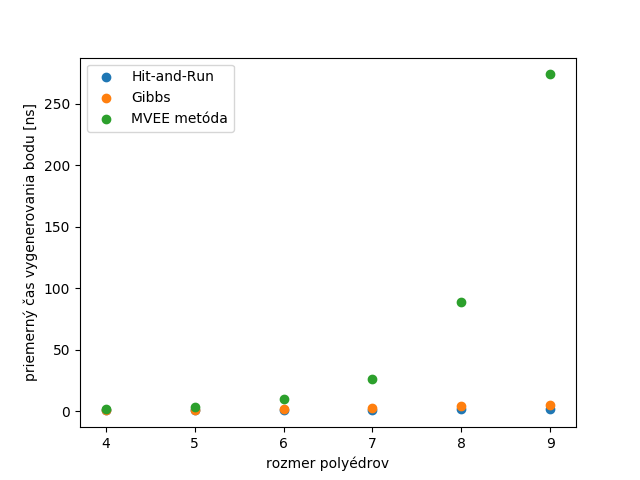
\includegraphics[width=\linewidth]{images/vsetky.png}
  \caption{Priemerný čas trvania všetkých metód}
  \label{fig:vsetky}
\end{figure}

Metóda MVEE pri vyššom počte rozmerov generuje body výrazne pomalšie ako Metropolis--Hastings metódy (viď \ref{fig:vsetky}). To môže byť jednak spôsobené zväčšením pomeru veľkostí V--reprezentácie ku H--reprezentácie alebo taktiež zväčšeniu pomeru objemov $\frac{\lambda(T_{MVEE})}{\lambda(S)}$. 
Ako druhý možný dôvod uveďme, že náš horný odhad $d^d$ očakávaného počtu generovaní (kde $d$ je počet rozmerov priestoru) podľa Johnovho elipsoidu nemusí byť tak voľný, ako sa na prvý pohľad zdá.\\

\begin{figure} [H]
	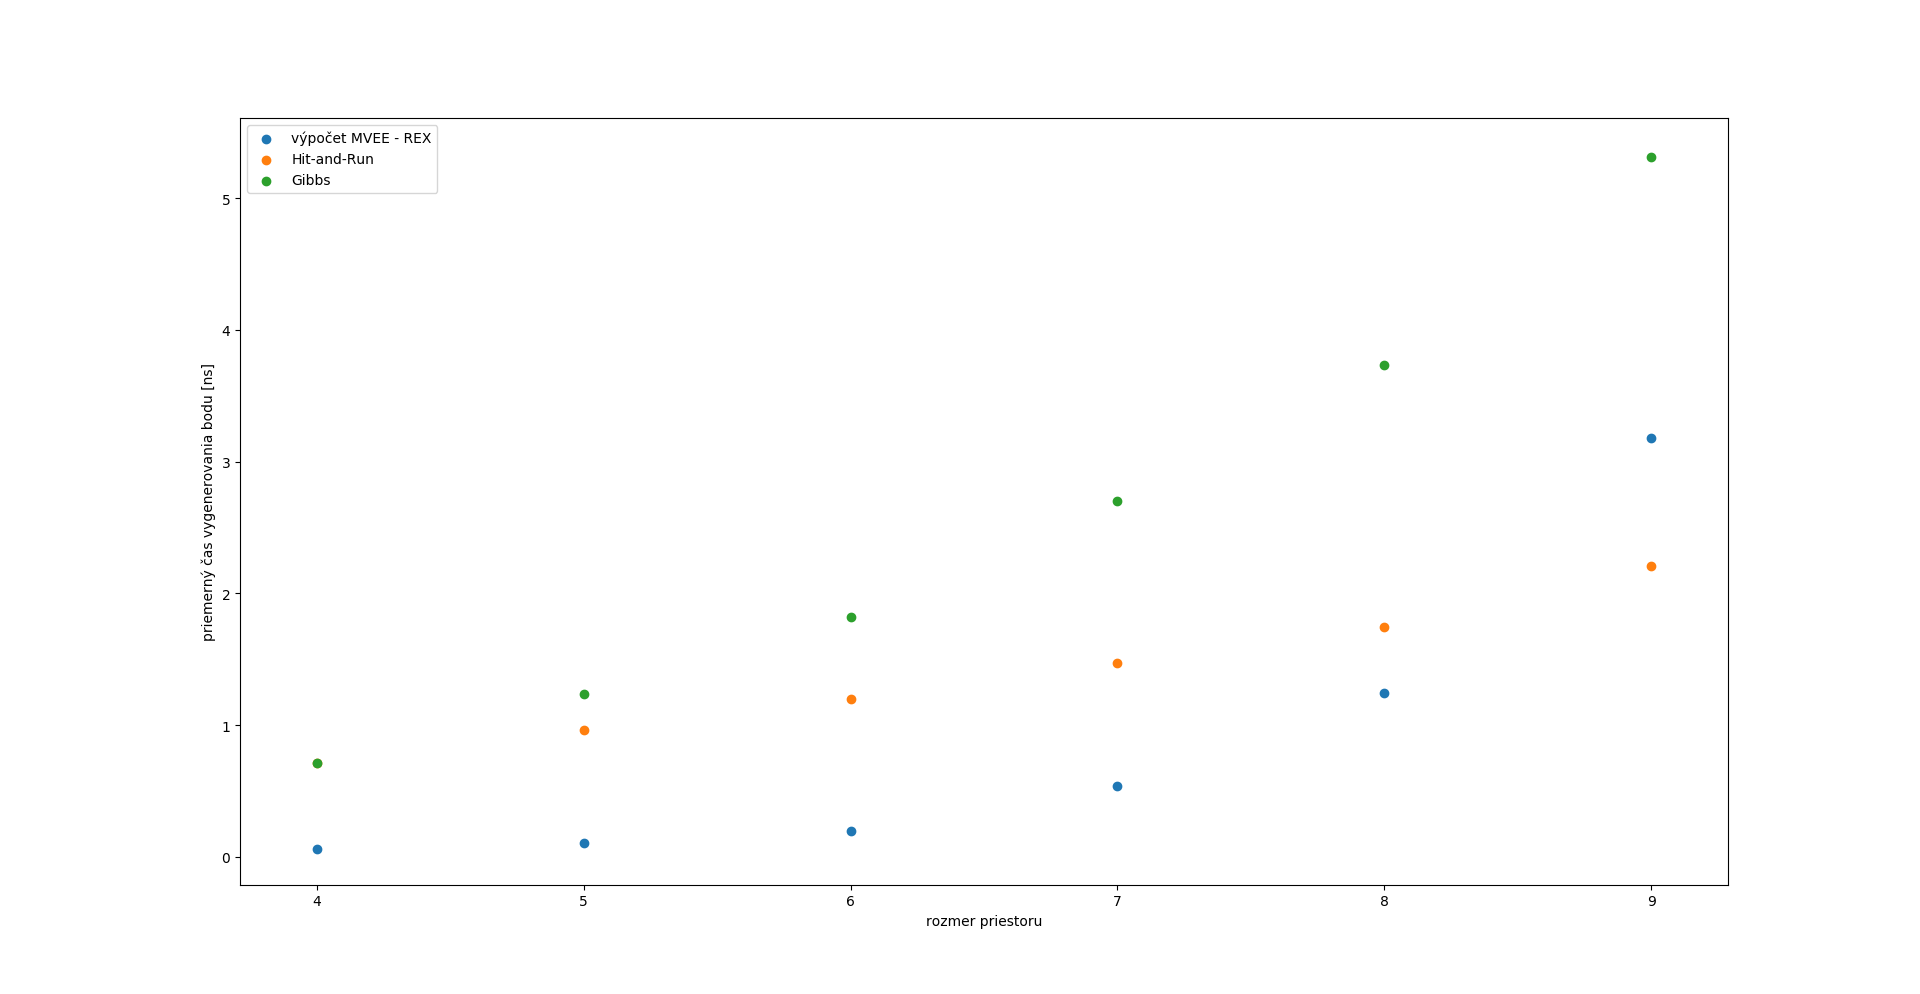
\includegraphics[width=\linewidth]{images/mh_rex.png}
	\caption{Porovnanie priemerného vygenerovania bodu Metropolis--Hasting metódou s výpočtom MVEE pomocou REX algoritmu vzhľadom na počet rozmerov priestoru \textbf{TODO vravi to nieco?}}
	\label{fig:mh_rex}
\end{figure}

\begin{figure} [H]
	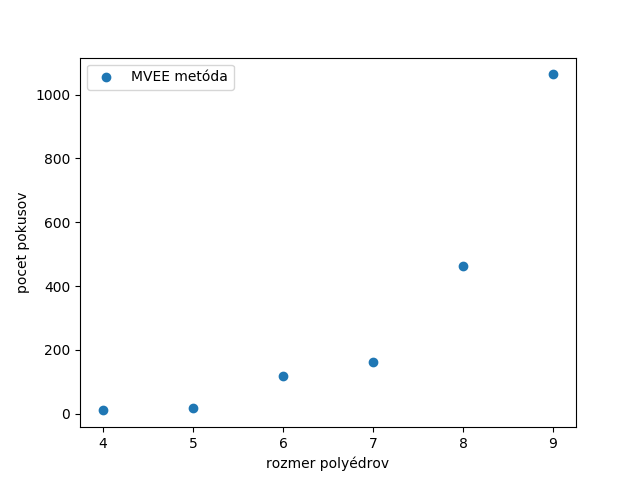
\includegraphics[width=\linewidth]{images/mvee_pokusy.png}
	\caption{Priemerný počet pokusov na nájdenie bodu v polyédri pomocou MVEE vzhľadom na počet rozmerov priestoru}
	\label{fig:mvee_pokusy}
\end{figure}

\begin{figure} [H]
	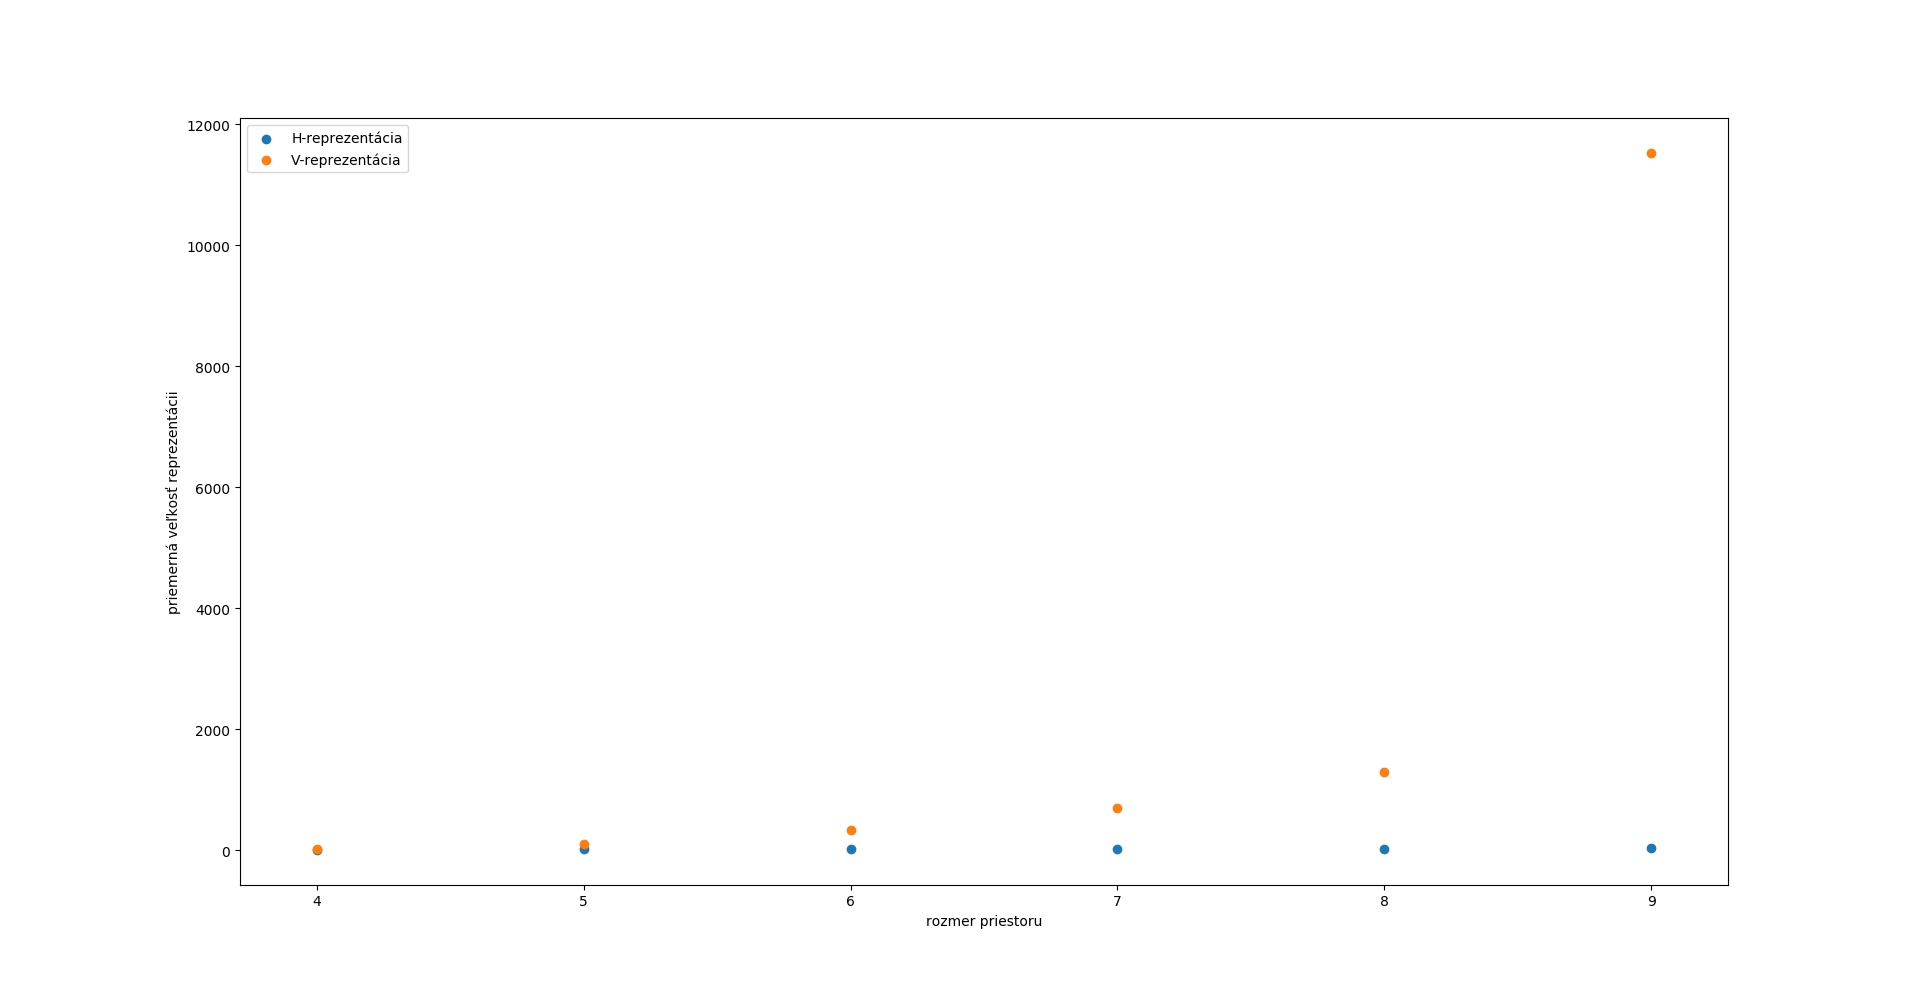
\includegraphics[width=\linewidth]{images/velkost_rep.png}
	\caption{Priemerná veľkosť reprezentácií polyédrov vzhľadom na počet rozmerov priestoru}
	\label{fig:velkost_rep}
\end{figure}

\begin{figure} [H]
	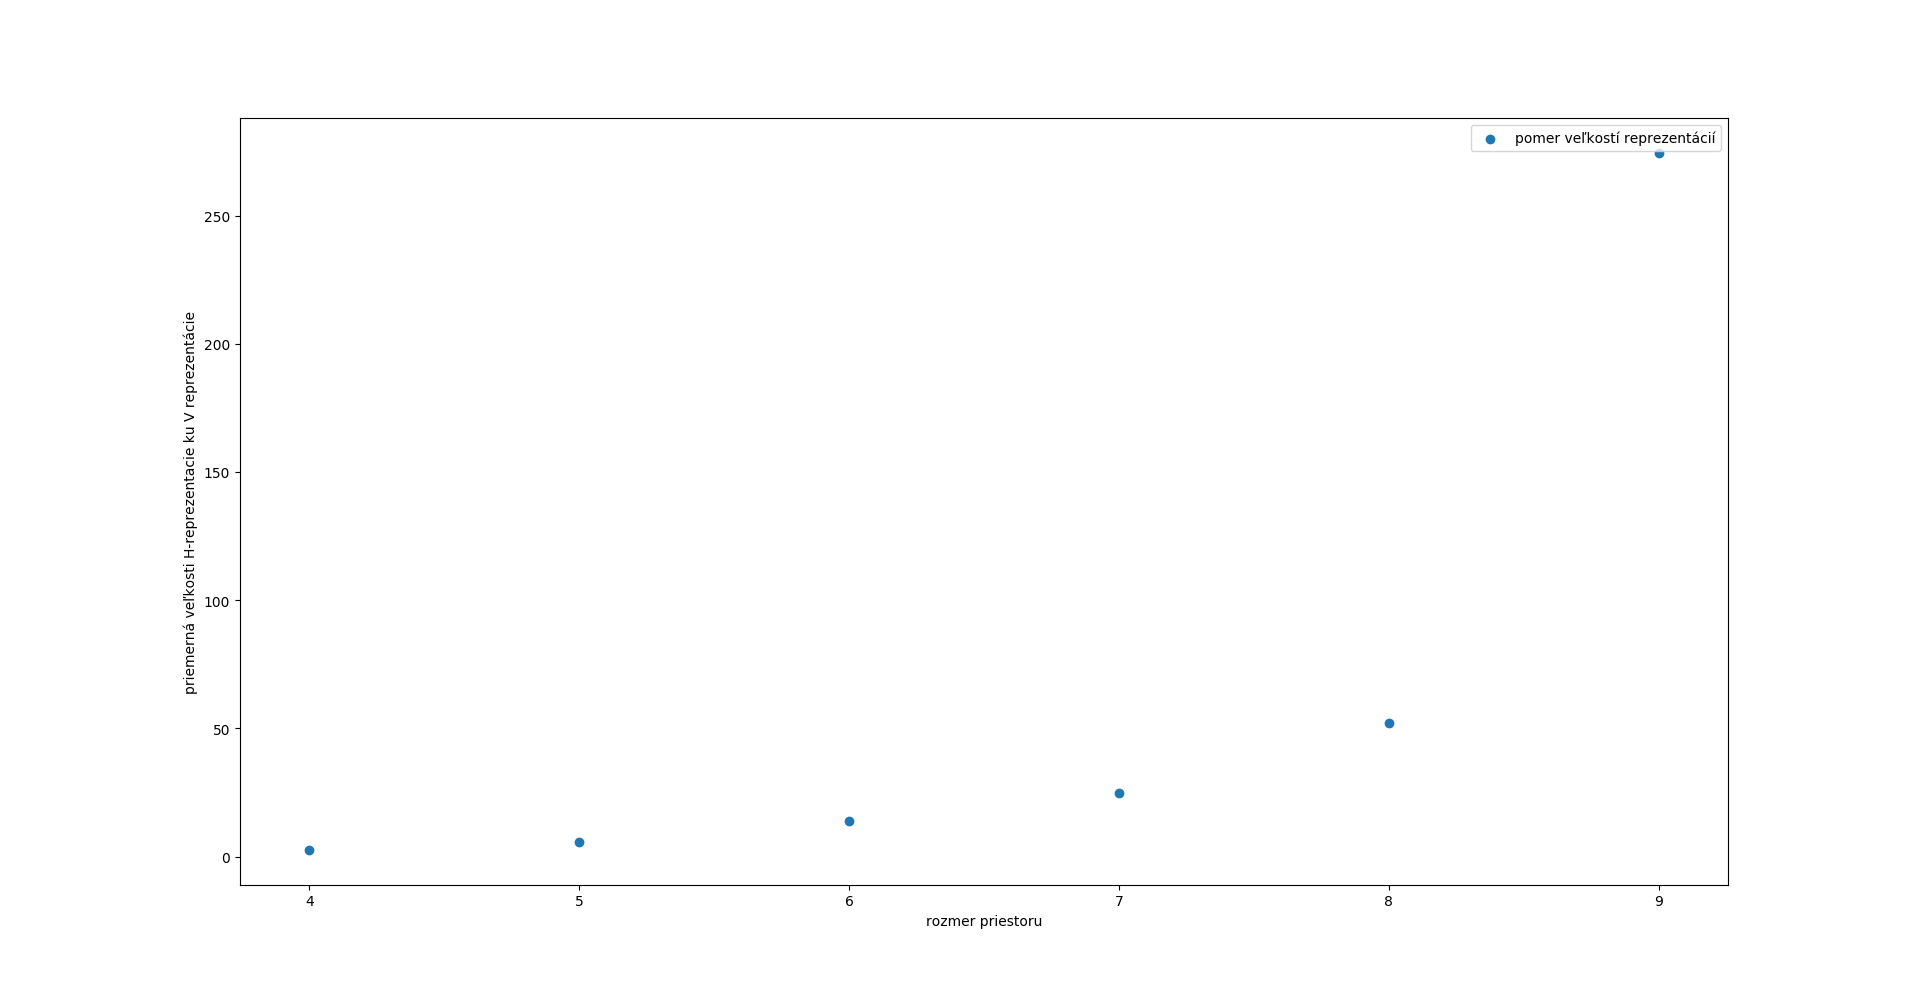
\includegraphics[width=\linewidth]{images/pomer_rep.png}
	\caption{Pomer veľkostí reprezentácii polyédrov vzhľadom na počet rozmerov priestoru}
	\label{fig:pomer_rep}
\end{figure}
